
\chapter{QuickMap : yet another NetGen-compatible map browser}

\begin{quote}

{\sl \bf{Note :} QuickMap is developed by Pierre-Yves Lucas as a geographic frontend to NetGen.}

\end{quote}

\label{sec:chapter5bis}

This chapter will present QuickMap, an evolution of the tool presented in chapter \ref{sec:chapter5}
to support precise geographic positions and easy map  browsing. 

A movie is available at {\tt http://wsn.univ-brest.fr/QuickMap/} that demonstrates 
the tool in action to describe and control field of sensors,  working
under the control of satellite.

QuickMap has also support for displaying 
buildings or obstacles representations extracted from OpenStreetMap databases. 
The present tools allow to interact with the more common public information systems 
such as Google map and OpenStreetMap. 

The map browser is a tool allowing to display various kind of maps and to represent 
locations of interest such as sensors set in the country. 
As this tool is developped on the same platform as NetGen, the procedures described 
in chapter \ref{sec:chapter1} will apply to access the software: 
\begin{itemize}
\item start a fresh image and ensure that the NetGen package is loaded with one of the last version (1.28.1.2.5 should work)
\item open the store dialog from VisualWorks main window menu bar
\item select QuickMap package 
\item select last version, and type load from the pop-up menu
\end{itemize}

\subsection{Short presentation}

Figure 
\ref{fig:initialQuickMapBrest} shows a view on a QuickMap windowi with a number
of control button on the left, and map display on the right.


\begin{figure}
\begin{center}
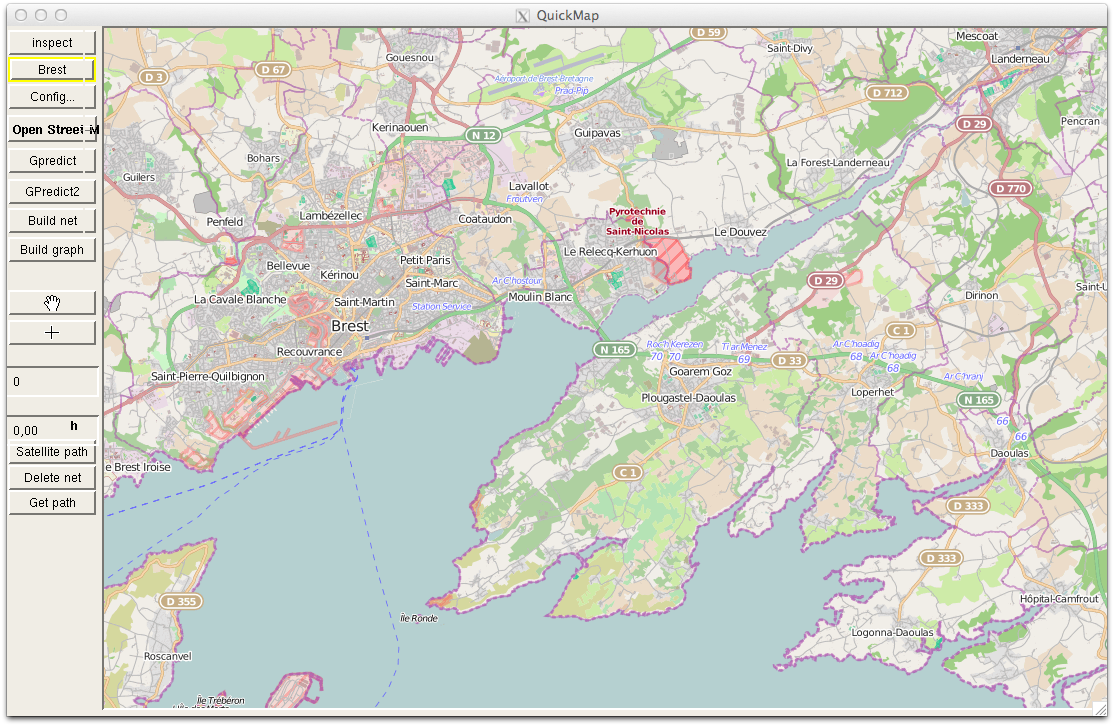
\includegraphics[width=10cm]{QuickMapSatBrest.png}
\caption{Initial view on QuickMap version for satelite control,
pointng to default Brest location. The user interface allows to move directly maps using
the hand cursor. The sensor wheel controls depth in the map system, here OpenStreetMap.}
\label{fig:initialQuickMapBrest}
\end{center}
\end{figure}

The movie proposed at  {\tt http://wsn.univ-brest.fr/QuickMap/} is a sequence representing 
the current tool status:

\begin{description}
\item  [Moving the map ]: shows horizontal and vertical moves on an OpenStreetMap map system. 
\item [Launching GPredict  ]: external software that allows to select satellite and pipe informations to QuickMap. 
\item [Following Satellite ]: these values are collected and presented on QuickMap, the red ball figures the selected satellite. 
\item [Specification of a sensor field]: some sensors are positioned in front of the satellite path.
\item [Building networks ]: build button ask computation of edges representing communication links establishment and disconnection.
\item [Network synthesis ]: using the old version of the browser, the communication ranges can be modified, then the problem is passed to NetGen for simulatioon (CUDA).
\item [System simulation ]:  satellite and sensors work together, synchronously. The distributed program start at the same step
on the ground and in the air. Bounding box for controlled sensor systems are computed and displayed.
\end{description}


